% ---------
% --------
%!TEX TS-program = pdflatex
%!TEX encoding = UTF-8 Unicode
%!TEX spellcheck = English (Aspell)

\documentclass[11pt]{article}
\usepackage{lucy,handout,graphicx}
\usepackage{fourier-orns}
\usepackage{mathtools}
\usepackage[normalem]{ulem} % either use this (simple) or
\usepackage{tikz}

\def\Cdot{\mathbin{\text{\normalfont \textbullet}}}
\def\Sym#1{\texttt{\color{BrickRed}#1}}
\def\BlueSym#1{\textbf{\texttt{\color{RoyalBlue}#1}}}
\allowdisplaybreaks

\begin{document}

\begin{center}
\Large\textbf{CSCI 332, Fall 2026}%
\\
\LARGE\textbf{Homework 8 (Part 2---Part 1 is on Prairie Learn)}%
\\[0.5ex]
\large Due Monday, October 26 Anywhere on Earth (6am Tuesday)
\end{center}

\bigskip
\hrule
\bigskip

\subsection*{Submission Requirements}
\begin{itemize}
    \item Type or clearly hand-write your solutions into a PDF format so that they are legible and professional. Submit your PDF on Gradescope. 
    \item Do not submit your first draft. Type or clearly re-write your solutions for your final submission. If your submission is not legible, we will ask you to resubmit.
    \item Use Gradescope to assign problems to the correct page(s) in your solution. If you do not do this correctly, we will ask you to resubmit.
\end{itemize}

\subsection*{Academic Integrity}

Remember, you may access \EMPH{any} resource in preparing your solution to the homework. However, you \EMPH{must}
\begin{itemize}
    \item write your solutions in your own words, and
    \item credit every resource you use (for example: ``Bob Smith helped me on
    this problem. He took this course at UM in Fall 2020''; ``I found a solution
    to a problem similar to this one in the lecture notes for a different
    course, found at this link: www.profzeno.com/agreatclass/lecture10''; ``Here is a link to the full transcript of my chat with ChatGPT about the problems on this HW''.)
    Ask if you need any clarifications about how to properly cite your sources!
\end{itemize}




\newpage
%----------------------------------------------------------------------
    
\headers{CSCI 332}{Homework 8 (due October 26)}{Fall 2026}


\begin{enumerate}
%\parindent 1.5em \itemsep 4ex plus 0.5fil

%----------------------------------------------------------------------

\item (0 points) List the resources you used for each problem in this homework. If you used no resources except
lecture notes and videos and the linked textbook, you can say ``none''. If you used
an AI tool, you should put a link to your full conversation here, and you must
use the
\href{https://umaal.org/files/teaching/csci332_fall2026/agents.md}{provided
prompt}
 to guide the AI to act
as a tutor, not an answer-provider.

You will be asked to resubmit your homework if this section is blank.

Remember that no matter what resources you consulted, you must write your solutions
\emph{in your own words}.

\item (2 points) Analyze the runtime of \textsc{WhateverFirstSearch} by
reporting upper bounds (big O) on the number of times the following lines
run, given an undirected graph $G$ with $|V|$ nodes and $|E|$ edges. For example,
line (0) runs $O(1)$ times. Then, using these observations, give a big O runtime for
WFS.

\begin{verbatim}
WFS(s):
  put s into the bag            (0)
  while the bag is not empty:
    take v from the bag         (3)
    if v is unmarked:
      mark v                    (2)
        for each edge {v,w}:
          put w into the bag    (1)
\end{verbatim}

\item (3 points) Snakes and Ladders is a classic board game, originating in
India no later than the 16th century. The board consists of an $n \times n$ grid
of squares, 
numbered consecutively from 1 to $n^2$, starting in the bottom left corner and
proceeding row by row from bottom to top, with rows alternating to the
left and right. Certain pairs of squares in this grid, always in different rows,
are connected by either “snakes” (leading down) or “ladders” (leading up).
Each square can be an endpoint of at most one snake or ladder.

You start with a token in cell 1, in the bottom left corner. In each move,
you advance your token up to $k$ positions, for some fixed constant $k$. If the
token ends the move at the top end of a snake, it slides down to the bottom
of that snake. Similarly, if the token ends the move at the bottom end of a
ladder, it climbs up to the top of that ladder.

Describe and analyze an algorithm to compute the smallest number of
moves required for the token to reach the last square of the grid.

\begin{center}
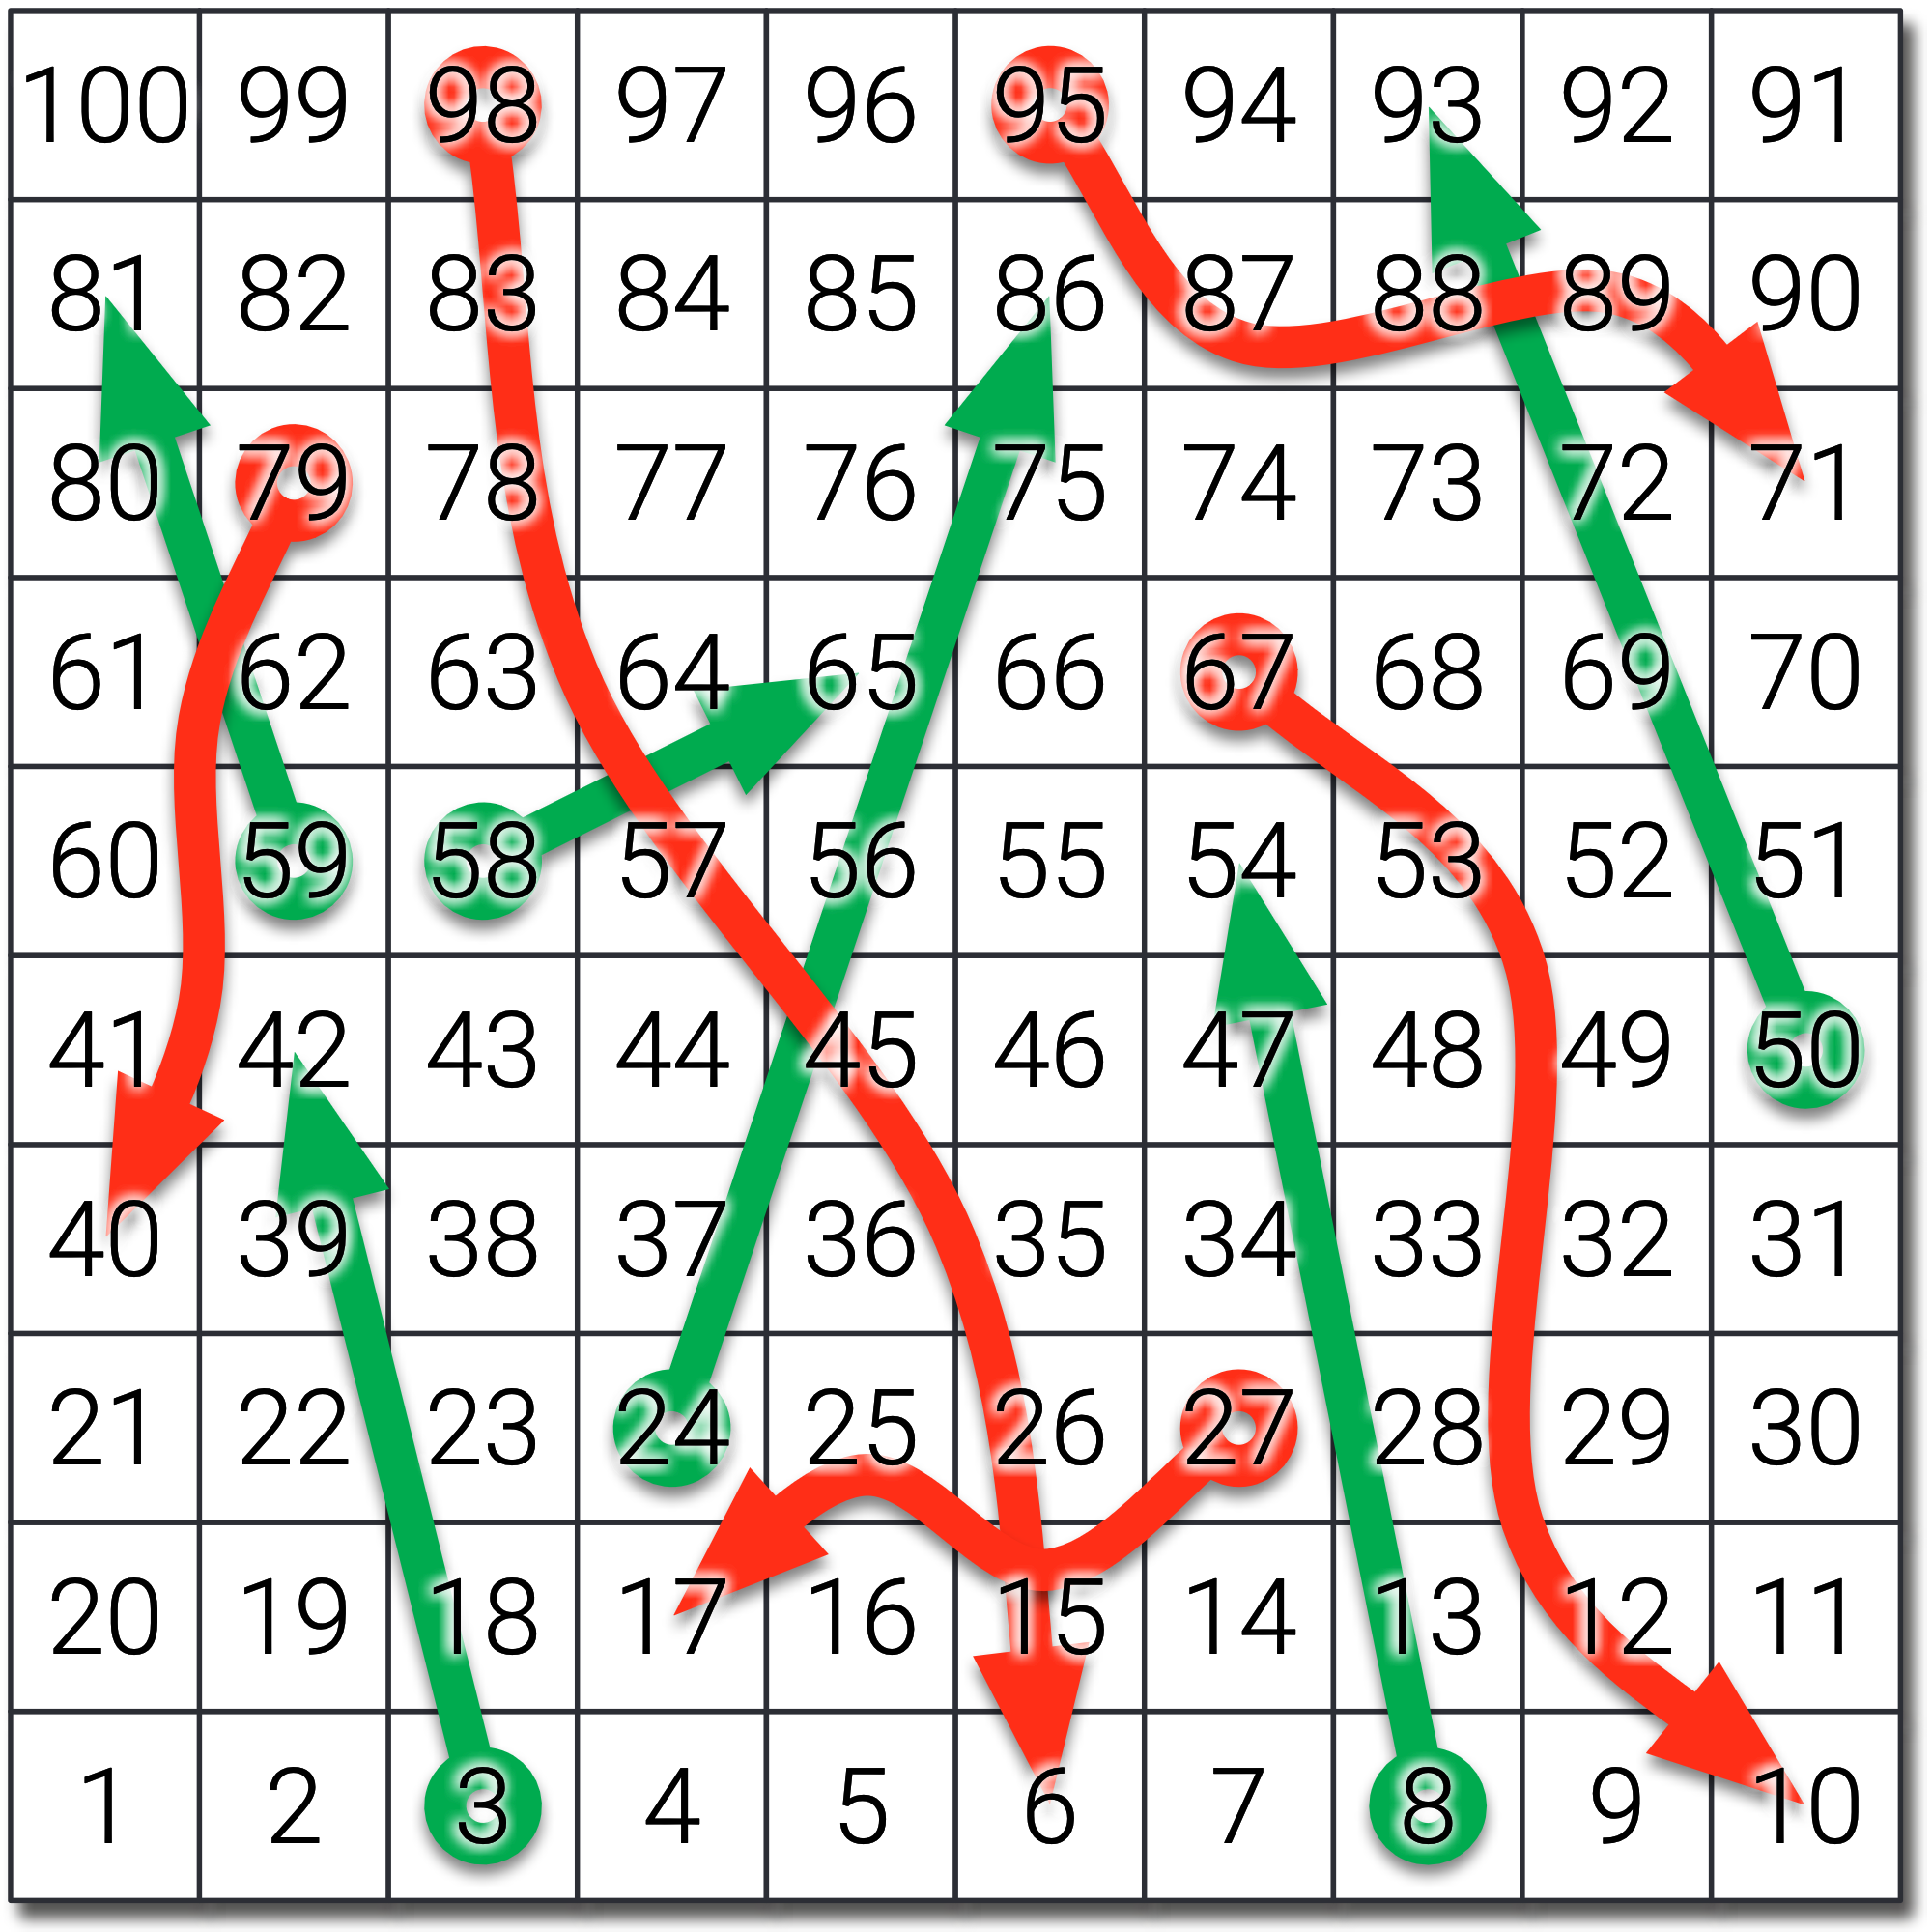
\includegraphics[width=0.55\linewidth]{snakes+ladders.png}
\\
\footnotesize\sffamily
An example of snakes and ladders.
\end{center}


\end{enumerate}
%%%%%%%%%%%%%%%%%%%%
\end{document}
